\appendix

\newgeometry{total={210mm,297mm},left=30mm,right=30mm,bindingoffset=5mm, top=25mm,bottom=25mm}
\begin{partwithabstract}{Appendix}
  Apendices to the document:
  \begin{enumerate}
    \item Details regarding the reproducability of this work.
    \item Agreement documents for use of the xVertSeg dataset.
    \item Addentum regarding the pre-defence and the seminars followed during this academic year.
  \end{enumerate}
\end{partwithabstract}
\restoregeometry


\chapter{Used software \& Reproducability of this research}

\section{Reproducability of the used environment}
The reproducability of this work has been ensured in several ways:
\begin{description}
  \item[Data]: All datasets used in this project are publically available. For some datasets, it is required to request permission, like the author of this work has done.
  \item[Software]: This project was performed completely in python, a publically available programming language. 
  All packages used are open-source.
  To reproduce this research, no software has to be purchased. 
  \item[Code]: Both code an text of this project can be found on a public \texttt{GitHub} repository: \url{https://github.com/JanAlexanderPersonal/MastatThesis.git}.
  \footnote{It is possible that small adaptations of the code are required to run it on other hardware. For example, to run it using a GPU with less internal memory it could be necessary to reduce the batch size.}. 
  \item[Docker]: The specific environment to run the code mentioned above can also be found in the mentioned GitHub repository in the form a dockerfile.
  It should be noted that this dockerfile requires a GPU that supports CUDA.   
\end{description}

The above mentioned aspects should allow other researchers to reproduce the results in this document.
This work makes use of parts of \textit{haven.ai} \footnote{This is a collection of libraries developed by the team of dr. I. Laradji to manage different experiments in deep learning research.} 
as a basis to manage different experiments.
These experiments are conducted using the deep learning library \textit{PyTorch}.
This tool is widely used in boty industry and academic research.
A list of other Machine Learning tools used in this work is provided below.
Table \ref{tab:UsedTools} is not an exhaustive list of all  python libraries used in this work.
It aims to list the more advanced tools, crucial for this work.

\begin{SCtable}[\sidecaptionrelwidth][h]
 
  \begin{tabular}{ p{2cm} l l } 
   \hline
   \hline
   \textbf{Library} & \textbf{version} & \textbf{reference}    \\
   \hline 
  Python & 3.8 & Programming language \\
   \hline
   \multicolumn{3}{c}{Deep learning and machine learning tools} \\
   \hline
   PyTorch & 1.7.1 & Deep learning library \\ 
   scikit-learn & 0.24.2 & Machine learning toolbox \\
   \hline
   \multicolumn{3}{c}{Tools to work with (medical) images} \\
   \hline
   SimpleITK & 2.0.2 & Library for medical images \\ 
   kornia & 0.2.0 & Computer vision library linked to torch \\
   scikit-image & 0.18.1 & Image manipulation library \\
   Pillow & 8.2.0 & Image manipulation\\
   \hline
   \multicolumn{3}{c}{Tools for matrix \& scientific computation} \\
   \hline
   numpy & 1.20.3 & matrix manipulation \\
   scipy & 1.6.3 & scientific calculation \\
   \hline
   \multicolumn{3}{c}{Result visualization} \\
   \hline
   matplotlib & 3.4.2 & data visualization \\ 
   seaborn & 0.11.1 & data visualization \\
   \multicolumn{3}{c}{Neural network experiment management} \\
   \hline
   haven &  & experiment management \\ 
   \hline
   \hline
  \end{tabular}
  \caption{Python libraries used. \label{tab:UsedTools}}

\end{SCtable}

Table \ref{tab:UsedTools} is not an exhaustive list of all libraries used in this work.
One can quickly dublicate the environment used in this work by building the \textit{Docker} environment defined in \texttt{dockerfiles} (part of the \texttt{GitHub} repository).

\section{Hardware\label{sec:hardware}}
The main hardware components of the device used for this work are listed below:

Intel® Core™ i7-9700 CPU @ 3.00GHz $\times$ 8 \\
RAM : 32 GB

\textsc{GPU}:\\
\hspace{5mm}GeForce RTX 2080 Ti (4352 CUDA cores)\\
\hspace{5mm}total memory 11264 MB\\
\hspace{5mm}CUDA version 11.2



\section{Other}
The formatting of this document, bringing Tufte layout elements in the \LaTeX{} memoir class, is based on the excelent post found on \url{https://tex.stackexchange.com/questions/275565/tufte-layout-in-painless-memoir}.
Didier Dufrasne gave a few very helpful tips for improving this layout.
The Neural network architecture illustrations were made using this project: \url{https://github.com/HarisIqbal88/PlotNeuralNet}.
The conceptual illustration of the neural network idea on page \pageref{fig:ann} is based on \url{https://tex.stackexchange.com/questions/153957/drawing-neural-network-with-tikz}.



\newgeometry{total={210mm,297mm},left=30mm,right=30mm,bindingoffset=5mm, top=25mm,bottom=25mm}
\chapter{Dataset agreements\label{seg:datasetagreement}}

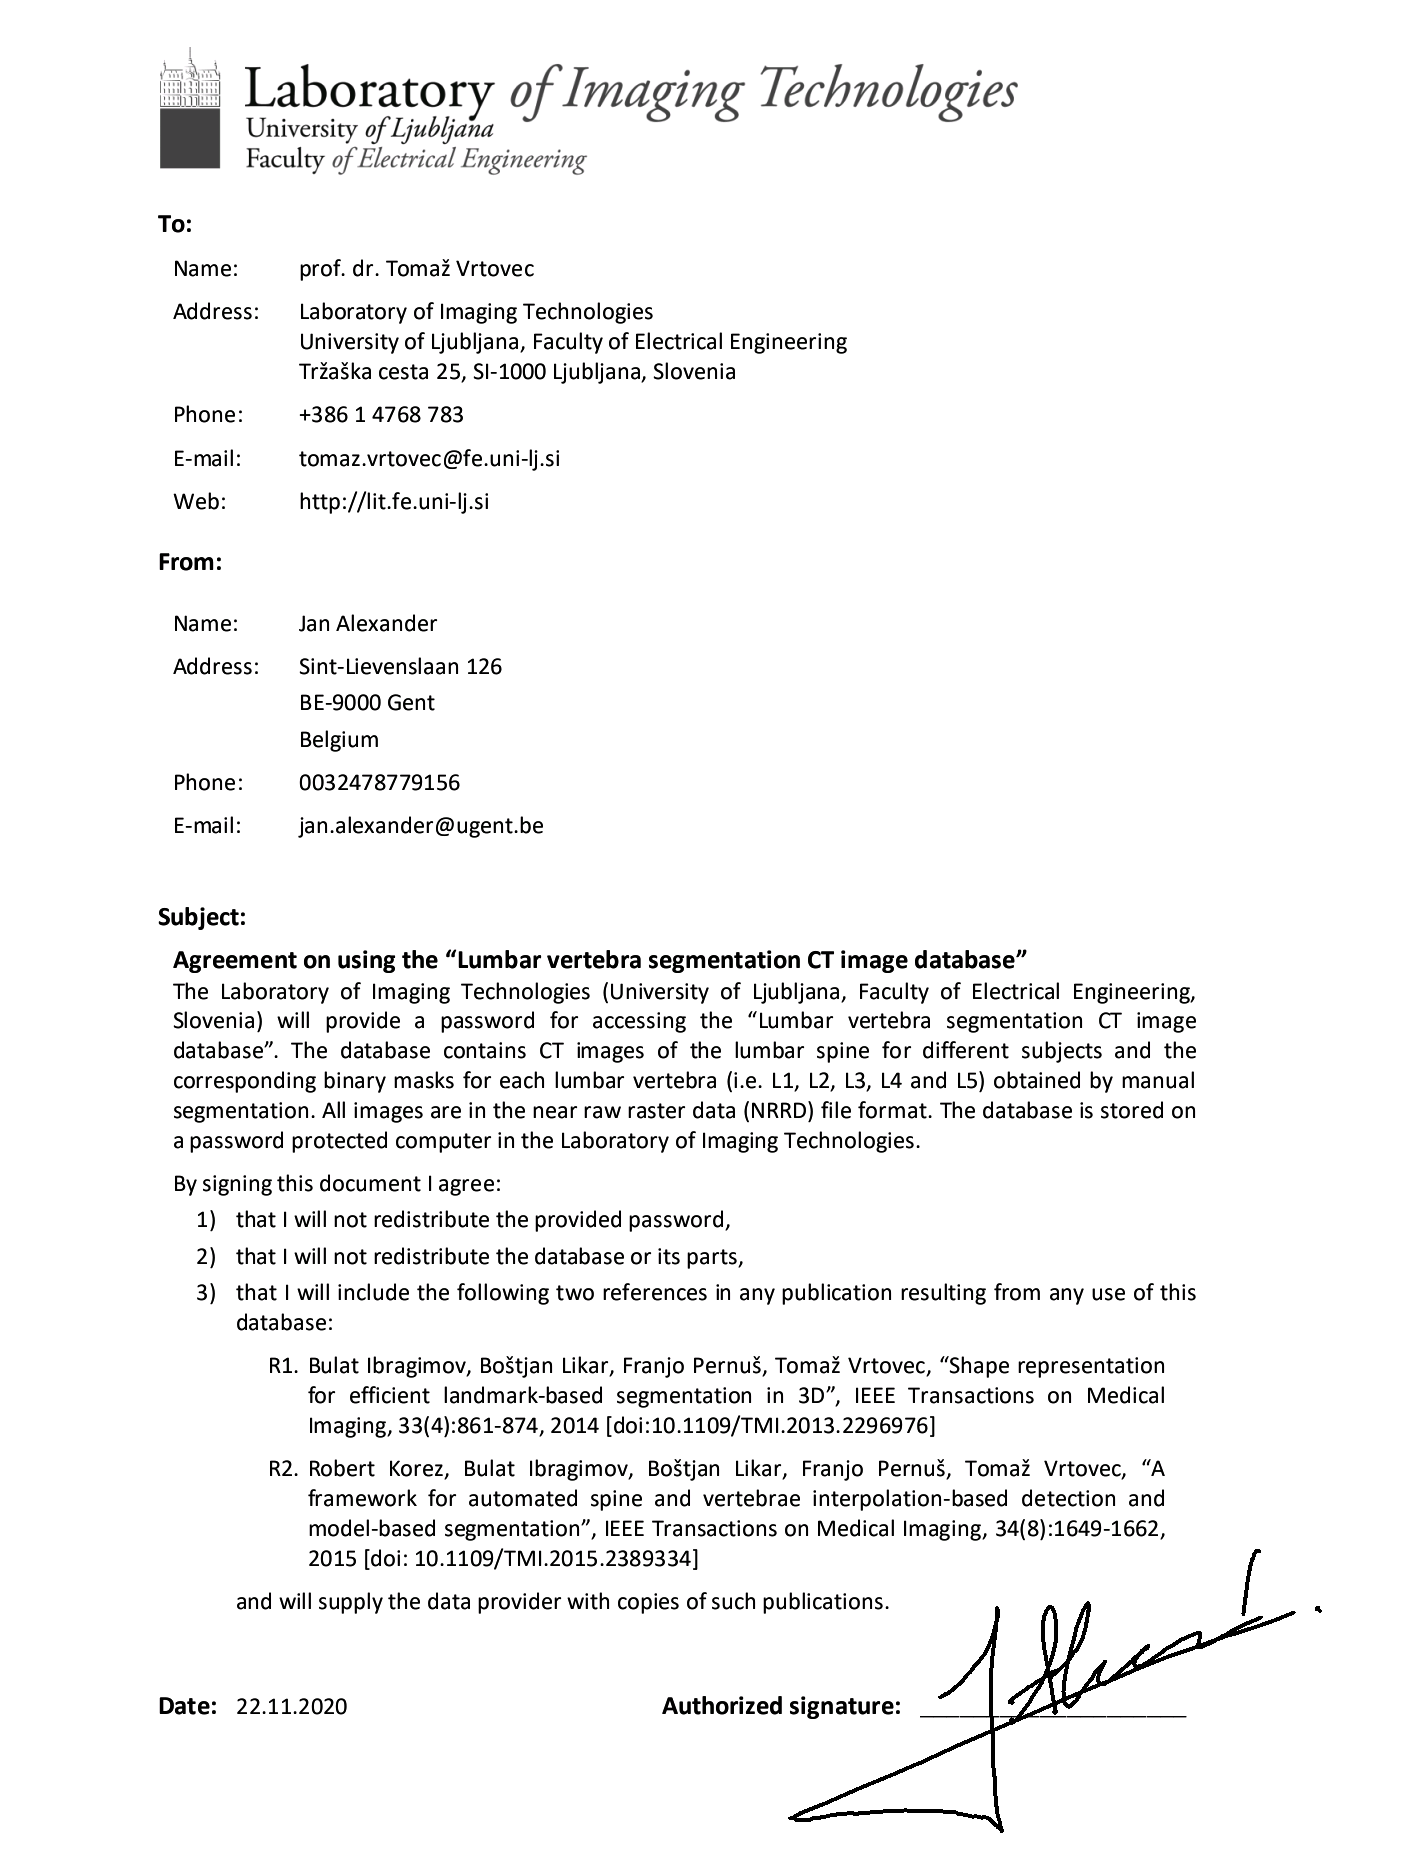
\includegraphics[width=17cm]{/home/thesis/images/AgreementxVertSeg.png}

\chapter{Predefence and seminars}
\par{
  On March 31$^st$, 2021 the concept of this work was presented in a poster session seated by Prof. Stijn Vansteelandt.
The poster used during this event is included on the next page for reference.
}



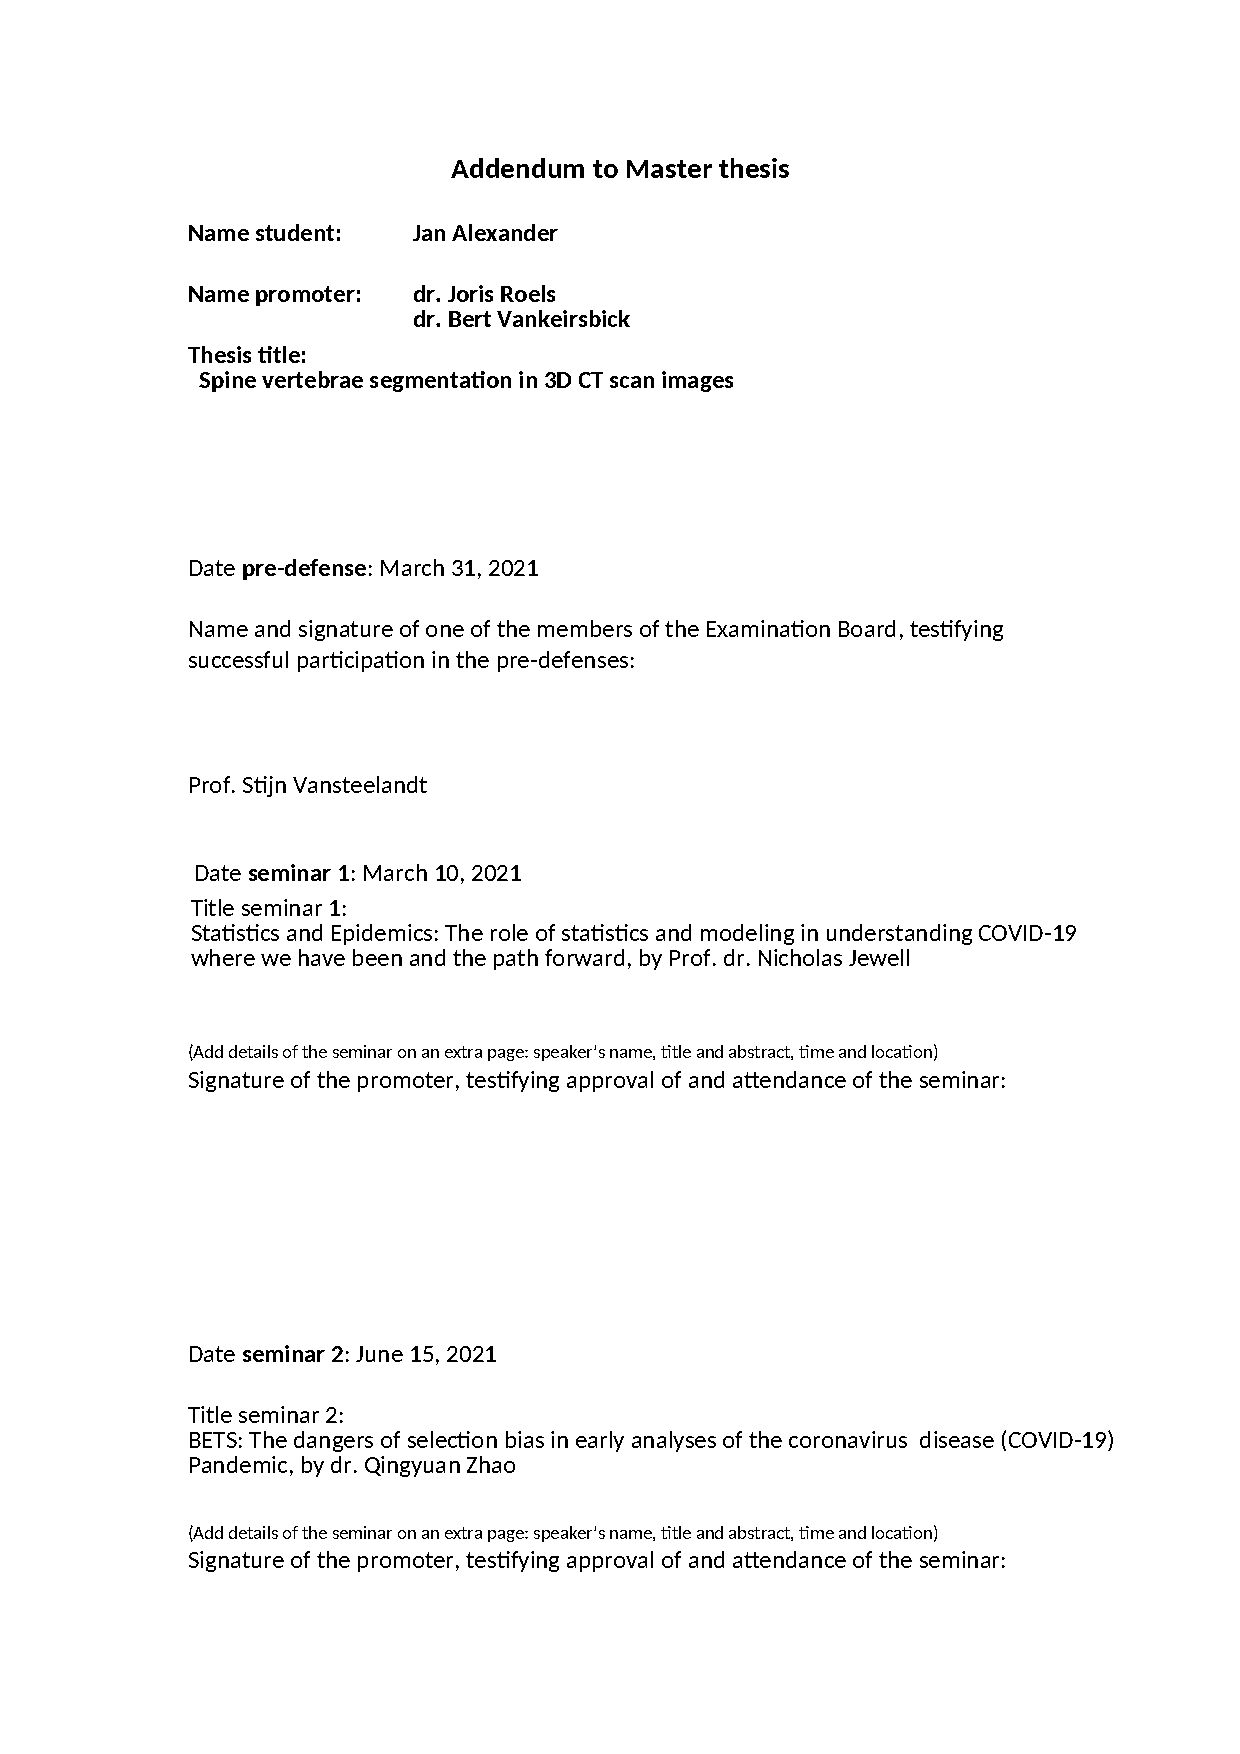
\includepdf[fitpaper=true, pages=-]{/home/thesis/images/Addendum_thesis_seminars.pdf}
\includepdf[fitpaper=true, pages=-]{/home/thesis/images/Poster_JanAlexander.pdf}
